\documentclass[11pt]{article}

\usepackage[final]{acl}
\usepackage{times}
\usepackage{latexsym}
\usepackage[T1]{fontenc}
\usepackage[utf8]{inputenc}
\usepackage{microtype}
\usepackage{inconsolata}
\usepackage{graphicx}
\usepackage{booktabs}
\usepackage{multirow}
\usepackage{amsmath}
\usepackage{xcolor}
\usepackage{adjustbox}

\newcommand{\gold}{\textsc{Amz-Gold}}
\newcommand{\dist}{\textsc{Amz-Dist}}

\title{Does Syntax Still Help? Dependency-Tree Graph Networks versus\\Transformers for Aspect-Based Sentiment on Amazon and Yelp Reviews}

\author{Author One \and Author Two \and Author Three \\
  Department, Institute \\
  \texttt{\{author1,author2,author3\}@institute.edu}}

\begin{document}
\maketitle

\begin{abstract}
Graph neural networks over dependency trees were, for a few years, the standard way to inject syntax into aspect-based sentiment classification. We revisit them under a single training protocol and compare a GCN, a GAT and a relation-aware GAT against a BiLSTM without a graph, a fine-tuned RoBERTa, and RoBERTa models with a dependency GNN on top. Besides the SemEval-2014 and MAMS benchmarks, we evaluate on Yelp reviews and on Amazon Reviews 2023 (Electronics), for which we build a distantly supervised training set from star ratings and a manually labelled test set of 225 aspect mentions drawn mostly from contrastive, multi-aspect sentences. With static word embeddings the dependency graph gives no reliable gain over the BiLSTM, although it is better than a random tree of the same size on Rest14. RoBERTa is 5 to 8 points more accurate than every GloVe model. Adding a dependency GNN to RoBERTa does not change average accuracy much on in-domain benchmarks, but it raises accuracy on sentences whose aspects carry different polarities by 12 to 18 points on Lap14 and on the Amazon test set, and the gain is consistent across seeds. It vanishes on MAMS, where every training sentence is of this kind. We also find that rating-based distant labels are only about 70\% correct and that models trained on them do not transfer to manually labelled Amazon data, while a laptop-domain model does. Finally, we run the pipeline over 97k Amazon reviews (588k aspect mentions) and report the accuracy and throughput trade-off between the two model families.
\end{abstract}

\section{Introduction}

Aspect-based sentiment classification (ABSC) asks for the polarity that a text expresses towards a given aspect term. In ``\textit{The battery life is great but the screen is too dim}'', the answer is positive for \textit{battery life} and negative for \textit{screen}. Sentence-level sentiment models cannot separate the two, and sequence models with attention \citep{wang-etal-2016-attention,tang-etal-2016-aspect} often attach an opinion word to the wrong aspect when the words are close in the surface string. A dependency parse makes the link explicit: \textit{dim} is two arcs away from \textit{screen} and three from \textit{battery life}. This observation led to a line of work that runs graph convolutional \citep{kipf2017semi} or graph attention \citep{velickovic2018graph} networks over the dependency tree \citep{zhang-etal-2019-aspect,sun-etal-2019-aspect,huang-carley-2019-syntax,wang-etal-2020-relational,li-etal-2021-dual}.

Most of these models were proposed when the encoder was a BiLSTM over GloVe vectors. Pre-trained transformers have since raised the baseline considerably, and \citet{dai-etal-2021-syntax} argued that much of what the parse provides is already present in RoBERTa. Two practical questions remain open for a practitioner who has to analyse large volumes of product and business reviews. First, is it worth parsing at all once a transformer is available, and if so, for which sentences? Second, the public ABSC benchmarks are small and come from 2014; real review platforms such as Amazon and Yelp have millions of reviews but almost no aspect-level labels. How far can one get with labels derived from star ratings, and how should such models be evaluated?

This report addresses both questions. Our contributions are:
(i) a controlled comparison of BiLSTM, GCN, GAT and relation-aware GAT encoders, a fine-tuned RoBERTa, and RoBERTa with a dependency GNN, trained with the same data, parser, model selection on a held-out development split, and multiple seeds;
(ii) a graph-structure ablation that separates the effect of syntax from the effect of simply having a sparse graph;
(iii) an Amazon Reviews 2023 setting with a distantly supervised training set, a 100-item audit of its label quality, and a manually labelled test set focused on contrastive sentences;
(iv) a breakdown of errors by sentence type and by syntactic versus linear distance between aspect and opinion word; and
(v) a corpus-scale run over 97k Amazon reviews that measures what the accuracy gains of a transformer cost in throughput.
All code, processed data, per-example predictions and a notebook that regenerates every table are released with the report.

\section{Related Work}

\paragraph{Attention and memory models.} Early neural ABSC models encode the sentence with an LSTM and let the aspect attend over the hidden states \citep{wang-etal-2016-attention} or over an external memory \citep{tang-etal-2016-aspect}. These models depend on the attention distribution finding the right opinion word, which is unreliable when several opinions appear in one sentence.

\paragraph{Dependency graph models.} ASGCN \citep{zhang-etal-2019-aspect} applies a GCN on top of a BiLSTM, weights tokens by their distance to the aspect, and reads out an aspect representation that attends back over the sentence. CDT \citep{sun-etal-2019-aspect} is a close variant. \citet{huang-carley-2019-syntax} use graph attention over the tree, and R-GAT \citep{wang-etal-2020-relational} reshapes the tree around the aspect and adds embeddings of the dependency relations. DualGCN \citep{li-etal-2021-dual} combines a syntactic and a semantic graph. Our GloVe models follow ASGCN closely and differ only in the graph layer, so that differences can be attributed to that layer.

\paragraph{Pre-trained transformers.} Fine-tuning BERT \citep{devlin-etal-2019-bert} as a sentence-pair classifier is a strong ABSC baseline, which can be improved further by domain post-training \citep{xu-etal-2019-bert}. \citet{dai-etal-2021-syntax} show that trees induced from a fine-tuned RoBERTa \citep{liu2019roberta} work as well as parser trees inside graph models, and that RoBERTa with an MLP head is already competitive with the graph models of the time. We extend this line by looking at where, within a test set, the parse still helps a transformer.

\paragraph{Data.} SemEval-2014 Task 4 \citep{pontiki-etal-2014-semeval} supplies the Rest14 and Lap14 benchmarks. MAMS \citep{jiang-etal-2019-challenge} was built so that every sentence contains at least two aspects with different polarities. Amazon Reviews 2023 \citep{hou2024bridging} is a large collection of product reviews with star ratings and no aspect labels. Using ratings or emoticons as noisy labels is an old idea for sentence-level sentiment \citep{go2009twitter}; we test how well it carries over to the aspect level.

\section{Data}
\label{sec:data}

Table~\ref{tab:data} summarises the datasets. All texts are tokenised and parsed with spaCy's \texttt{en\_core\_web\_lg} 3.8 model \citep{honnibal2020spacy}. Long reviews are cropped to the sentence that contains the aspect (with one neighbouring sentence when the sentence has fewer than six tokens), and the cropped text is parsed again so that each example is a single rooted tree.

\begin{table}[t]
\centering
\small
\setlength{\tabcolsep}{4pt}
\begin{adjustbox}{max width=\columnwidth}
\begin{tabular}{lrrrrr}
\toprule
 & train & dev & test & len & mixed \\
\midrule
Rest14 & 3,246 & 362 & 1,120 & 19.0 & 19.5 \\
Lap14 & 2,095 & 233 & 638 & 17.8 & 15.2 \\
MAMS & 11,186 & 1,332 & 1,336 & 28.9 & 99.9 \\
Yelp & 727 & 81 & 245 & 18.2 & 9.0 \\
\dist & 6,805 & 837 & 858 & 18.3 & 0.0 \\
\gold & n/a & n/a & 225 & 23.6 & 41.3 \\
\bottomrule
\end{tabular}
\end{adjustbox}
\caption{Number of aspect instances per split, mean test sentence length in tokens, and the share of test instances (\%) whose sentence contains aspects with different polarities.}
\label{tab:data}
\end{table}

\paragraph{Benchmarks.} Rest14 and Lap14 are the SemEval-2014 restaurant and laptop sets, and MAMS is used with its official splits. For Rest14 and Lap14 we hold out 10\% of the training sentences as a development set, splitting by sentence so that aspects of the same sentence stay together. Restaurants are the domain closest to Yelp and laptops the one closest to Amazon Electronics.

\paragraph{Yelp.} We use the Yelp ABSC set distributed with PyABSA \citep{yang2023pyabsa}: full Yelp reviews with aspect terms and polarity labels. After cropping it is a small and skewed set (727 training instances, 64\% positive, 7\% neutral), which turned out to matter for the transformer results.

\paragraph{Amazon Reviews 2023, distant labels (\dist).} We use a 100k-review sample of the Electronics category of Amazon Reviews 2023. The reviews have star ratings only. After HTML clean-up and de-duplication we shuffle the reviews, take 40k for the distant set, and keep a disjoint 3k for annotation. Aspect terms are taken from a lexicon mined on the 161k parsed sentences: the 400 most frequent nouns and the 200 most frequent compound-noun bigrams (\textit{battery life}, \textit{sound quality}, \textit{customer service}), after removing a hand-written stoplist of nouns that are rarely opinion targets (\textit{time}, \textit{thing}, \textit{review}, \textit{husband}, \dots). A sentence that mentions at least one lexicon aspect is labelled as follows. All its aspects are \textit{positive} if the review has four or five stars and the VADER compound score \citep{hutto2014vader} of the sentence is at least 0.5; \textit{negative} if the review has one or two stars and VADER is at most $-0.3$; and \textit{neutral} if the sentence contains no word from the VADER lexicon and no evaluative adjective. Sentences with a contrast marker (\textit{but}, \textit{however}, \textit{although}, \dots) are removed, since their aspects may disagree. Out of 105,904 sentences with an aspect, 17,657 were removed as contrastive and 49,389 matched no rule. Negative sentences are the scarce class (3,712 instances against 42,056 positive), so we cap the classes at 3,000 negative, 2,000 neutral and 3,500 positive instances and split by review into 80/10/10.

\paragraph{Audit of the distant labels.} To estimate label quality we labelled 100 random instances of the \dist{} test split by hand, without looking at the distant label. Eleven candidates were not opinion targets at all (for example \textit{life} in ``\textit{for the life of me}''). On the remaining 89, the distant label was correct in 62 cases (69.7\%). The precision is similar for the three classes (positive 68\%, negative 72\%, neutral 69\%). Nearly all errors involve the neutral class: an incidental noun inherits the sentiment of its sentence (17 cases), or a neutral-looking sentence still expresses an opinion through a word that VADER does not know (9 cases). Only one positive label should have been negative. Rating and sentence sentiment therefore get the polarity direction right but cannot tell which noun the opinion is about, and that is the part ABSC is about.

\paragraph{Manually labelled Amazon test set (\gold).} From the 3k held-out reviews we sampled candidate aspect mentions with the same lexicon, over-sampling sentences that contain a contrast marker and at least two aspects. Each candidate was labelled for the polarity expressed towards it, following the SemEval-2014 guidelines; comparison objects (``\textit{faster than my old stick}'') receive the polarity expressed towards them, and mere mentions are neutral. Of 260 candidates, 35 were rejected as non-targets, leaving 225 instances in 135 sentences (64 positive, 36 negative, 125 neutral). The set is deliberately hard: two thirds of the instances come from multi-aspect sentences with a contrast marker, and 41\% from sentences whose aspects have different polarities. It shares no review and no sentence with \dist.

\section{Models}
\label{sec:models}

\subsection{Graph construction}
For a sentence of $n$ tokens we build a symmetric adjacency matrix $A \in \{0,1\}^{n \times n}$ from the parse, with self-loops. For the ablations in Section~\ref{sec:ablation} we replace it with (a) a chain graph linking each token to its neighbours, (b) a random tree with the same number of nodes and edges, and (c) a fully connected graph. For the relation-aware model, each edge also carries the label of its dependency arc, out of 45 ClearNLP labels plus a self-loop label.

\subsection{GloVe-based models}
All four models share the same encoder and readout. Tokens are embedded with frozen 300-dimensional GloVe vectors \citep{pennington-etal-2014-glove} (6B release) concatenated with a 30-dimensional POS-tag embedding, and encoded by a BiLSTM with 300 units per direction.

\textbf{BiLSTM+Att} has no graph layer. The sum of the aspect's hidden states is used as a query that attends over all hidden states, and the attended vector is classified.
\textbf{GCN} follows ASGCN \citep{zhang-etal-2019-aspect}: two layers of $h^{(l+1)} = \mathrm{ReLU}(\tilde{A}\, (p \odot h^{(l)}) W^{(l)})$, where $\tilde{A}$ is the row-normalised adjacency and $p$ down-weights tokens far from the aspect. The aspect positions of the last layer are summed and used as the attention query.
\textbf{GAT} replaces each GCN layer by four-head graph attention restricted to the tree neighbours \citep{velickovic2018graph}.
\textbf{R-GAT} adds, for every edge, a learned per-head bias for its dependency label to the attention logits and a label embedding to the message, in the spirit of \citet{wang-etal-2020-relational}. We do not re-root the tree at the aspect.

Two details of the GAT turned out to matter. Our first version followed the attention aggregation with an extra linear projection, a residual connection and layer normalisation. It trained much more slowly than the GCN and on MAMS did not get past 55\% development accuracy. Removing the extra projection (so that the layer has the same output form as the GCN), applying the same position weights, and initialising the attention vectors to zero (so that the layer starts as mean aggregation over neighbours) fixed this. All GAT numbers in this report use the corrected layer.

\subsection{Transformer-based models}
\textbf{RoBERTa} is a fine-tuned RoBERTa-base \citep{liu2019roberta} that reads the pair ``\texttt{<s>} sentence \texttt{</s></s>} aspect \texttt{</s>}'' and classifies the first token. Because our compute environment had no access to the HuggingFace Hub, we extracted the RoBERTa-base weights shipped inside spaCy's \texttt{en\_core\_web\_trf} pipeline and converted them to the HuggingFace format. We verified that the converted encoder reproduces spaCy's hidden states (maximum absolute difference $5 \cdot 10^{-6}$). These weights were further trained by spaCy on OntoNotes tagging, parsing and NER, so they are not identical to the original checkpoint.
\textbf{RoBERTa+GCN} and \textbf{RoBERTa+R-GAT} take the last-layer state of the first sub-word of every word, project it to 384 dimensions, run two GCN or R-GAT layers over the parse, mean-pool the aspect nodes, and classify the concatenation of this vector with the \texttt{<s>} state.

\subsection{Training protocol}
GloVe models are trained with Adam (learning rate $10^{-3}$, weight decay $10^{-5}$, batch size 32, dropout 0.5 on embeddings and 0.3 after each graph layer) for up to 30 epochs, with early stopping after 8 epochs without improvement. Transformer models use AdamW \citep{loshchilov2019decoupled} with learning rate $2 \cdot 10^{-5}$ for the encoder and $10^{-3}$ for the new layers, batch size 16, 10\% linear warm-up, and four epochs (three on MAMS). In all cases the checkpoint with the highest sum of development accuracy and macro-F1 is evaluated once on the test set. We never select on test data; many published ABSC numbers report the best test epoch, which explains part of the gap between our numbers and the original papers (ASGCN reports 80.8\% on Rest14; our GCN reaches 79.1\%). GloVe models were run with three seeds. Because of the cost of CPU fine-tuning, transformer models were run with two seeds on Rest14, Lap14 and Yelp and with one seed on MAMS and \dist. Significance is assessed with a paired bootstrap over test instances \citep{berg-kirkpatrick-etal-2012-empirical} (5,000 resamples), using each instance's correctness averaged over seeds. All experiments ran on a 4-core CPU, 137 training runs in total.

\section{Results}

\subsection{Main comparison}

\begin{table*}[t]
\centering
\small
\begin{adjustbox}{max width=\textwidth}
\begin{tabular}{lcccccc}
\toprule
 & Rest14 & Lap14 & MAMS & Yelp & \dist & Lap14 $\rightarrow$ \gold \\
\midrule
BiLSTM+Att & 78.96 / 68.38 & 70.59 / 64.48 & 77.97 / 76.88 & 84.35 / 61.05 & 93.36 / 92.89 & 51.26 / 50.36 \\
GCN & 79.08 / 69.99 & 69.28 / 64.26 & 78.44 / 77.39 & 84.76 / 64.53 & 94.09 / 93.58 & 48.00 / 48.08 \\
GAT & 78.51 / 67.36 & 68.76 / 62.28 & 77.92 / 77.08 & 83.40 / 61.98 & 95.26 / 94.91 & 43.85 / 43.68 \\
R-GAT & 79.14 / 69.13 & 70.48 / 64.78 & 78.47 / 77.38 & 84.49 / 63.87 & 94.44 / 93.99 & 46.07 / 46.19 \\
\midrule
RoBERTa & 84.02 / 74.69 & 77.66 / 72.76 & \textbf{83.46} / \textbf{83.08} & 81.02 / 51.92 & 95.69 / 95.34 & 59.11 / 57.32 \\
RoBERTa+GCN & \textbf{84.42} / \textbf{75.98} & \textbf{78.68} / \textbf{74.20} & 83.08 / 82.68 & \textbf{84.69} / 55.18 & \textbf{96.27} / \textbf{96.09} & \textbf{64.22} / \textbf{63.50} \\
RoBERTa+R-GAT & 84.11 / 75.57 & 78.13 / 73.94 & 83.23 / 82.83 & 83.67 / 57.64 & 95.45 / 95.19 & 63.11 / 61.86 \\
\bottomrule
\end{tabular}
\end{adjustbox}
\caption{Test accuracy / macro-F1 (\%). GloVe models: mean of three seeds. Transformer models: mean of two seeds on Rest14, Lap14, Yelp and Lap14$\rightarrow$\gold, one seed on MAMS and \dist. Seed standard deviations are 0.4 to 2.4 points for accuracy (Appendix~\ref{app:std}).}
\label{tab:main}
\end{table*}

Table~\ref{tab:main} gives the main results.

\textit{The pre-trained encoder matters far more than the graph.} RoBERTa is 4.9 to 7.1 points more accurate than the best GloVe model on Rest14, Lap14 and MAMS, and the gap in macro-F1 is larger still on Lap14 and MAMS. On \gold, the laptop-trained transformers beat the laptop-trained GloVe models by 8 to 20 points.

\textit{On top of a GloVe BiLSTM, the dependency graph gives no reliable gain.} The four GloVe models differ by at most 1.8 points on any benchmark, which is of the same size as the seed variation. None of the GCN or R-GAT versus BiLSTM differences on the human-labelled sets is significant (the smallest $p$ is 0.25). R-GAT is better than GAT on every human-labelled set, by 0.6 to 2.2 points, so the relation labels do carry some information, but not enough to beat the model without a graph.

\textit{On top of RoBERTa, the graph gives small average gains in-domain.} RoBERTa+GCN is 0.4 points better than RoBERTa on Rest14 and 1.0 point better on Lap14 ($p = 0.27$ and $0.18$), and on MAMS both hybrids are slightly worse than RoBERTa (by 0.4 points for GCN and 0.2 for R-GAT, $p = 0.70$ and $0.64$). The picture changes on Yelp and on \gold. On Yelp, plain RoBERTa is the weakest model: with 727 training instances and only 49 neutral ones it never predicts the neutral class, and its accuracy (81.0) is below the GloVe models. The hybrids recover (84.7 and 83.7, $p < 0.001$ and $p = 0.03$). On \gold, RoBERTa+GCN gains 5.1 points over RoBERTa ($p = 0.02$) and RoBERTa+R-GAT 4.0 points ($p = 0.07$). Section~\ref{sec:fine} shows where these gains come from.

\subsection{Does the graph need to be syntactic?}
\label{sec:ablation}

\begin{figure}[t]
\centering
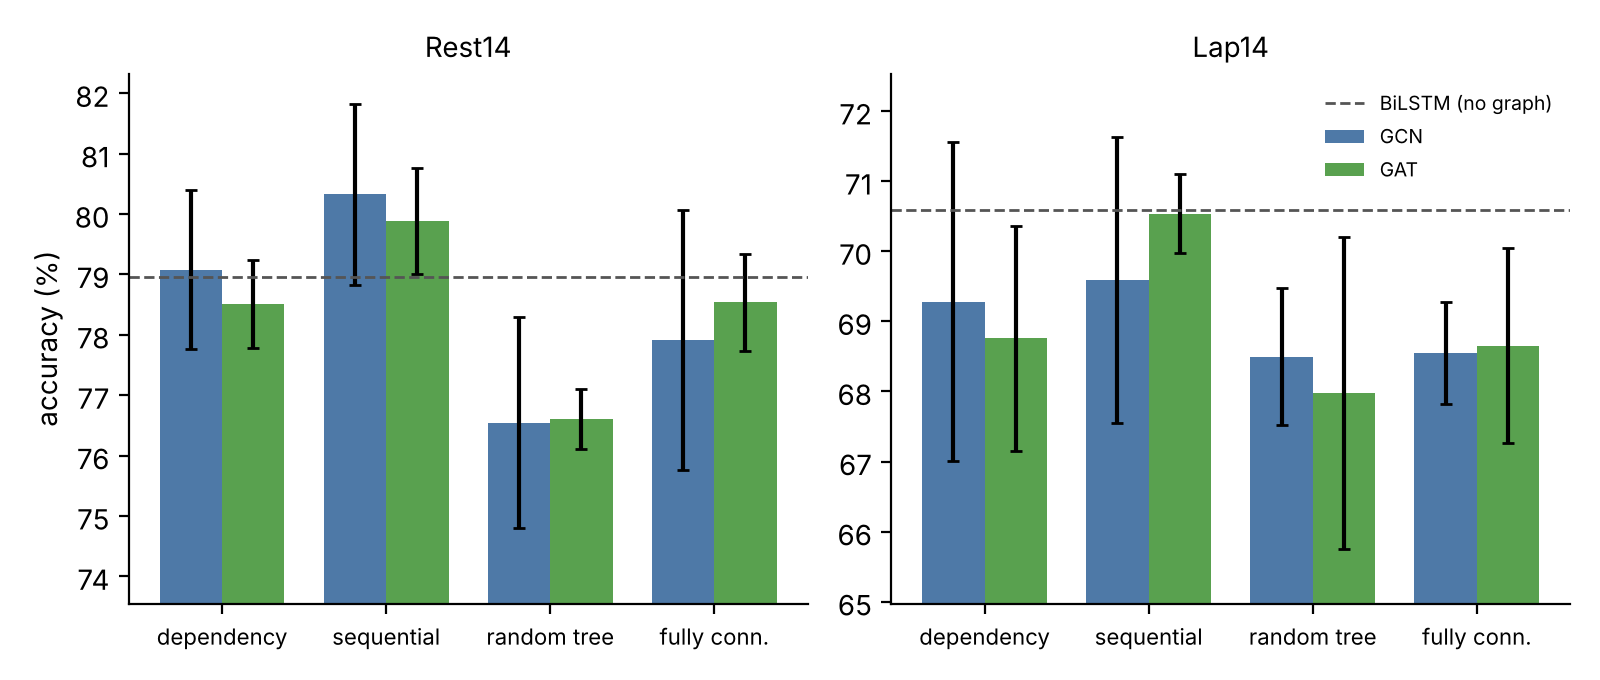
\includegraphics[width=\columnwidth]{figures/ablation_graph.png}
\caption{Test accuracy of GCN and GAT (GloVe) with different graphs, mean and standard deviation over three seeds. The dashed line is the BiLSTM without a graph.}
\label{fig:ablation}
\end{figure}

\begin{table}[t]
\centering
\small
\setlength{\tabcolsep}{3.5pt}
\begin{adjustbox}{max width=\columnwidth}
\begin{tabular}{lcccc}
\toprule
 & \multicolumn{2}{c}{Rest14} & \multicolumn{2}{c}{Lap14} \\
graph & GCN & GAT & GCN & GAT \\
\midrule
dependency & 79.1 / 70.0 & 78.5 / 67.4 & 69.3 / 64.3 & 68.8 / 62.3 \\
chain & \textbf{80.3} / \textbf{70.9} & \textbf{79.9} / \textbf{69.5} & \textbf{69.6} / 63.7 & \textbf{70.5} / \textbf{65.1} \\
random tree & 76.6 / 64.8 & 76.6 / 64.8 & 68.5 / 62.7 & 68.0 / 62.3 \\
complete & 77.9 / 67.7 & 78.5 / 67.5 & 68.6 / 62.3 & 68.7 / 62.4 \\
\midrule
no graph & \multicolumn{2}{c}{79.0 / 68.4} & \multicolumn{2}{c}{70.6 / 64.5} \\
\bottomrule
\end{tabular}
\end{adjustbox}
\caption{Graph-structure ablation, accuracy / macro-F1 (\%), three seeds.}
\label{tab:ablation}
\end{table}

Figure~\ref{fig:ablation} and Table~\ref{tab:ablation} replace the parse with other graphs while keeping everything else fixed. On Rest14 the dependency tree is clearly better than a random tree with the same number of edges (79.1 vs.\ 76.6 for GCN, 70.0 vs.\ 64.8 macro-F1), and for the GCN also better than a complete graph. So the parse does contain useful structure, and an arbitrary sparse graph actually hurts. However, the chain graph, which only connects adjacent words, is as good as or better than the tree on both datasets (80.3 for GCN on Rest14). Since the BiLSTM already encodes word order, a chain graph mostly adds a few extra local smoothing steps, and that seems to be all the GCN contributes in this setting. On Lap14 the differences between graphs are within seed variation. Varying the number of GCN layers between one and four on the parse changes accuracy by less than 1.3 points on either dataset (Appendix~\ref{app:layers}).

Our reading is that with a BiLSTM encoder, the useful part of the inductive bias is locality, and the parse only helps in so far as most dependency arcs are short. This agrees with \citet{dai-etal-2021-syntax}, who found that the choice of tree matters little once the encoder is strong.

\subsection{Where does syntax help?}
\label{sec:fine}

\begin{table}[t]
\centering
\small
\setlength{\tabcolsep}{3pt}
\begin{adjustbox}{max width=\columnwidth}
\begin{tabular}{lrcccc}
\toprule
 & $n$ & BiLSTM & RoB. & +GCN & +R-GAT \\
\midrule
\multicolumn{6}{l}{\textit{mixed-polarity sentences}} \\
Rest14 & 218 & 63.6 & 67.2 & 68.8 & \textbf{69.7} \\
Lap14 & 97 & 58.4 & 44.3 & 59.8 & \textbf{61.9} \\
Yelp & 22 & \textbf{77.3} & 54.5 & 61.4 & 63.6 \\
MAMS & 1334 & 77.9 & \textbf{83.4} & 83.1 & 83.2 \\
Lap14$\rightarrow$\gold & 93 & 49.5 & 46.8 & 59.1 & \textbf{62.4} \\
\midrule
\multicolumn{6}{l}{\textit{contrast marker in sentence}} \\
Lap14 & 70 & 55.2 & 60.0 & 59.3 & \textbf{62.9} \\
Lap14$\rightarrow$\gold & 141 & 47.0 & 49.6 & \textbf{59.6} & \textbf{59.6} \\
\midrule
\multicolumn{6}{l}{\textit{opinion word $\geq$3 arcs from aspect}} \\
Lap14 & 152 & 61.8 & 71.4 & 70.4 & \textbf{72.4} \\
Lap14$\rightarrow$\gold & 96 & 54.9 & 54.2 & 62.0 & \textbf{64.1} \\
\bottomrule
\end{tabular}
\end{adjustbox}
\caption{Accuracy (\%) on subsets of the test data, averaged over seeds. RoB.\ = RoBERTa.}
\label{tab:fine}
\end{table}

Averages hide where the models differ. Table~\ref{tab:fine} splits the test sets into subsets that should need syntax: instances from sentences whose aspects have different polarities, sentences with a contrast marker, and instances whose nearest opinion word (any word in the VADER lexicon with $|$valence$|\geq 1$) is three or more dependency arcs away.

On mixed-polarity sentences, adding a dependency GNN to RoBERTa raises accuracy from 44.3 to 59.8 (GCN) and 61.9 (R-GAT) on Lap14, and from 46.8 to 59.1 and 62.4 on \gold. These are the largest effects in the study, and they are not a seed artefact: on Lap14, plain RoBERTa scores 42.3 and 46.4 on this subset with its two seeds, while the hybrids score between 56.7 and 64.9; on \gold{} the ranges are 44.1 to 49.5 and 59.1 to 64.5. On Rest14 the subset gain is small and depends on the seed (one RoBERTa seed scores 70.2, above RoBERTa+GCN). On MAMS, where nearly all training sentences are mixed, RoBERTa alone is as good as both hybrids (83.4 vs.\ 83.1 and 83.2). We interpret this as a data-quantity effect. Rest14 has more than twice as many mixed-polarity training instances as Lap14 (812 vs.\ 385), and MAMS has over eleven thousand, so the transformer has enough examples to learn which opinion belongs to which aspect. With fewer such examples, or under a domain shift as with \gold, the parse supplies the missing prior.

The GloVe graph models do not show the same benefit. On Lap14 mixed-polarity sentences they are 6 to 12 points \emph{worse} than the BiLSTM, and on \gold{} they are 4 to 7 points worse. Their readout attends over BiLSTM states using the graph-smoothed aspect vector as a query, and in the examples we inspected this query was often dominated by the strongest opinion word of the sentence, whichever aspect it belonged to. The demo in the released notebook shows a typical case: for ``\textit{The sound quality is amazing, although the ear cushions get uncomfortable after an hour}'', the GloVe R-GAT used in Section~\ref{sec:scale} puts 99\% of its attention for \textit{ear cushions} on \textit{amazing} and predicts positive, while RoBERTa+GCN predicts positive and negative correctly.

\begin{figure*}[t]
\centering
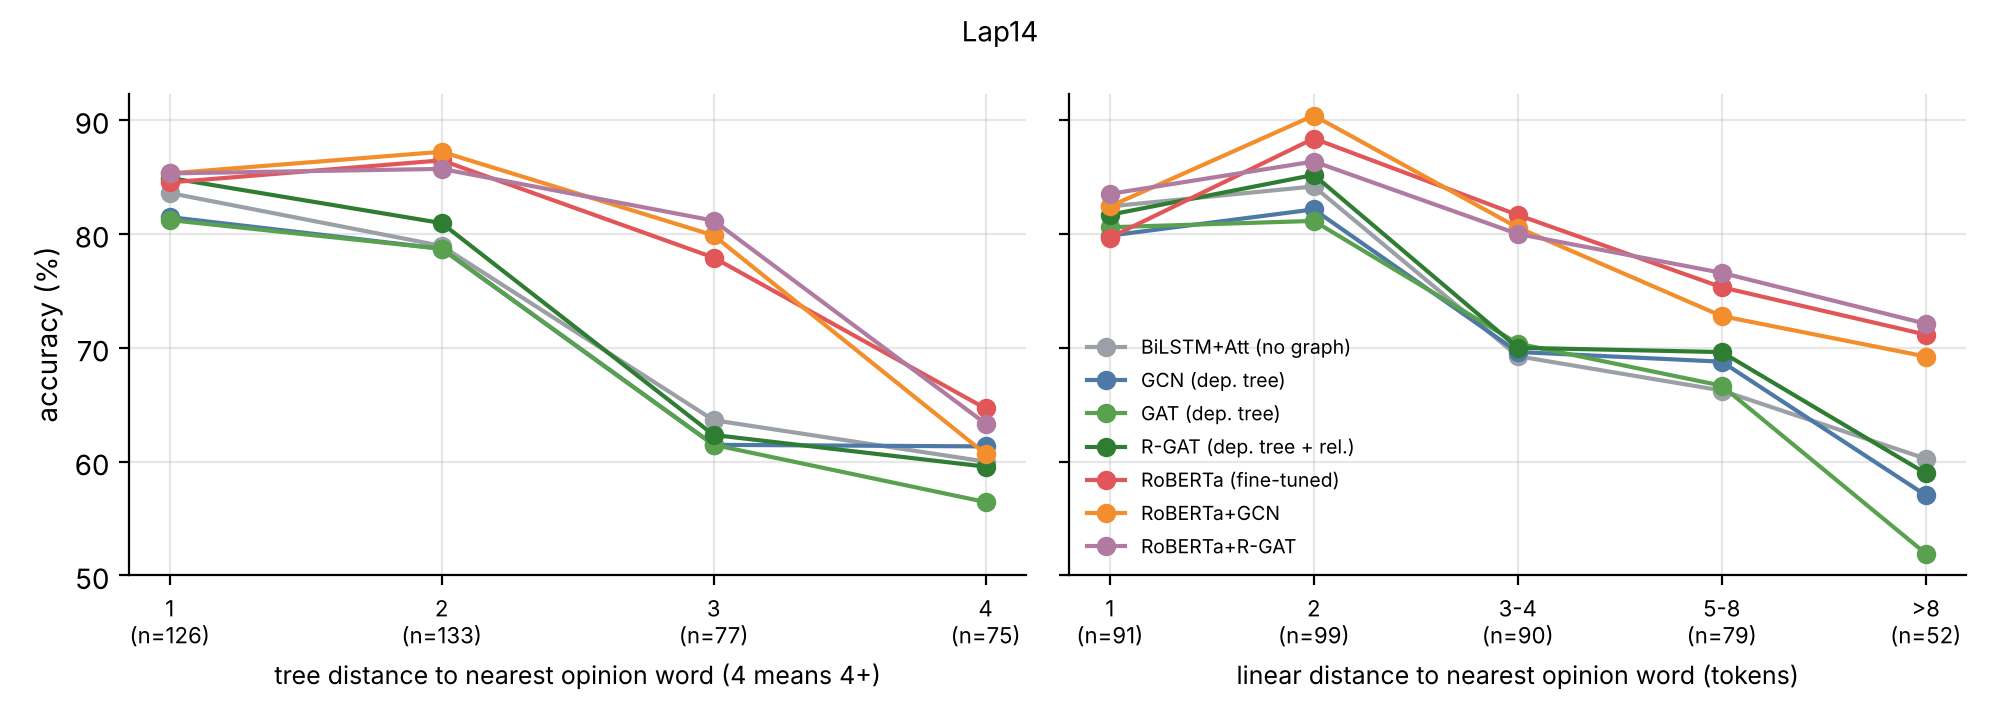
\includegraphics[width=0.82\textwidth]{figures/distance_lap14.png}
\caption{Lap14 accuracy as a function of the dependency distance (left) and the linear distance (right) between the aspect and its nearest opinion word, averaged over seeds.}
\label{fig:distance}
\end{figure*}

Figure~\ref{fig:distance} plots accuracy against the distance between aspect and nearest opinion word. All models degrade with distance, and the GloVe models degrade faster: they lose about 20 points between one and three arcs, the transformers about 5. At three arcs the hybrids are 2 to 3 points ahead of plain RoBERTa. At four or more arcs, where the parse is also least reliable, all transformers are around 60 to 65\%.

\subsection{Distant supervision and transfer}

\begin{table}[t]
\centering
\small
\setlength{\tabcolsep}{3pt}
\begin{adjustbox}{max width=\columnwidth}
\begin{tabular}{lcccc}
\toprule
train $\rightarrow$ test & BiLSTM & R-GAT & RoB. & +GCN \\
\midrule
\dist{} $\rightarrow$ \dist & 93.4 & 94.4 & 95.7 & 96.3 \\
\dist{} $\rightarrow$ \gold & 49.5 & 49.8 & 51.1 & 54.2 \\
Lap14 $\rightarrow$ \gold & 51.3 & 46.1 & 59.1 & \textbf{64.2} \\
\dist{} $\rightarrow$ Lap14 & 64.9 & 65.8 & 68.2 & 68.3 \\
Lap14 $\rightarrow$ \dist & 66.7 & 70.6 & 79.6 & 75.7 \\
\midrule
Rest14 $\rightarrow$ Yelp & 84.9 & 85.6 & 88.0 & 86.9 \\
Yelp $\rightarrow$ Rest14 & 70.3 & 72.4 & 75.3 & 75.5 \\
\bottomrule
\end{tabular}
\end{adjustbox}
\caption{Accuracy (\%) across training and test sets.}
\label{tab:transfer}
\end{table}

Table~\ref{tab:transfer} shows how the distant labels behave. Every model reaches 93 to 96\% on the \dist{} test split, far above the roughly 70\% label accuracy measured by our audit. The models have learnt the labelling heuristic, which is easy: sentiment words decide polarity and their absence decides neutrality. On \gold{} the same models score 49 to 54\%, which is below the 55.6\% obtained by always predicting \textit{neutral} (their macro-F1 of 47 to 52 is above the 23.8 of that baseline, so they are not useless, but close). A model trained on 2,095 human-labelled laptop sentences does much better on Amazon (59.1 for RoBERTa, 64.2 for RoBERTa+GCN), even though laptops are only one of many product types in the Electronics category. Training a GloVe R-GAT on the union of Lap14 and \dist{} did not help either (48.9\% on \gold). For this task, a small set of correct aspect-level labels from a neighbouring domain is worth more than several thousand rating-derived ones.

The restaurant results point the same way. A model trained on Rest14 is better on the Yelp test set (88.0 for RoBERTa, 89.2 for RoBERTa+R-GAT) than any model trained on the Yelp training set itself (at most 84.8). In the reverse direction, Yelp to Rest14, the dependency GNNs transfer better than the BiLSTM (72.4 to 73.0 vs.\ 70.3), the only setting where the GloVe graph models are clearly ahead.

\subsection{Corpus-scale analysis and cost}
\label{sec:scale}

\begin{table}[t]
\centering
\small
\setlength{\tabcolsep}{4pt}
\begin{adjustbox}{max width=\columnwidth}
\begin{tabular}{lrrr}
\toprule
model & params & ex/s & \gold \\
\midrule
BiLSTM+Att & 1.5M & 1,458 & 51.3 \\
GCN & 2.2M & 539 & 48.0 \\
R-GAT & 2.3M & 682 & 46.1 \\
RoBERTa & 124.1M & 73 & 59.1 \\
RoBERTa+GCN & 124.6M & 74 & 64.2 \\
\midrule
\multicolumn{4}{l}{\textit{full pipeline on Amazon, 4 CPU cores}} \\
R-GAT, 97k reviews & \multicolumn{3}{l}{2,207 mentions/s, 223 reviews/s} \\
RoBERTa+GCN, 10k reviews & \multicolumn{3}{l}{77 mentions/s, 11 reviews/s} \\
\bottomrule
\end{tabular}
\end{adjustbox}
\caption{Trainable parameters, test-time throughput (instances per second on CPU, batch 64; GloVe models measured with one thread, transformers with four), and accuracy on \gold{} (trained on Lap14). The lower part reports end-to-end throughput including parsing.}
\label{tab:cost}
\end{table}

To see what the models cost on real volumes of data, we ran the full pipeline (cleaning, sentence splitting and parsing with four spaCy processes, aspect extraction with the mined lexicon, batched inference) over the 97,487 non-empty reviews of the Amazon sample. This yields 499,928 sentences and 588,417 aspect mentions of 600 distinct aspect terms. With a GloVe R-GAT (trained on Lap14 plus \dist), parsing took 154 seconds and inference 267 seconds, or 2,207 mentions per second. Because the GloVe vectors are frozen during training, the vocabulary can be extended at inference time; 23k of the 40k unseen word types were found in GloVe. RoBERTa+GCN processed 77 mentions per second, 28 times slower, so we ran it on the first 10k reviews only. Table~\ref{tab:cost} puts these figures next to accuracy.

Without aspect-level labels for the whole corpus we validate the output against star ratings. For each review we average $+1$ (positive), $0$ and $-1$ (negative) over its aspect mentions and correlate this score with the rating. On the same 10k reviews the Spearman correlation is 0.39 for the GloVe R-GAT and 0.48 for RoBERTa+GCN (0.41 for the R-GAT over all 80,558 reviews with at least one mention). The R-GAT saw rating-derived labels during training, which makes its correlation partly circular; RoBERTa+GCN never saw a rating and still correlates better. The two models agree on 62\% of the mentions. The aggregate picture is plausible: \textit{value}, \textit{price}, \textit{quality} and \textit{color} are the most positive frequent aspects, and \textit{battery}, \textit{software}, \textit{button} and \textit{instructions} are the only frequent aspects (2,000 or more mentions) with more negative than positive mentions (Figure~\ref{fig:aspects} in the appendix).

For a practitioner this gives a clear trade-off. A GloVe graph model can tag hundreds of reviews per second on a laptop CPU, but on hard sentences it is barely better than a constant prediction. A transformer is an order of magnitude slower and much more accurate, and adding a parse to it costs almost nothing at inference time (the parser runs at over 600 reviews per second) while improving exactly the sentences that matter for aspect-level analysis.

\section{Discussion}

The question in our title has a qualified answer. With static embeddings, a dependency GNN in the ASGCN style does not beat a well-tuned BiLSTM on any of our test sets, and a chain graph does at least as well as the parse. Some of the gains reported in earlier work are probably due to model selection on the test set, which we avoid. Syntax becomes useful in combination with a pre-trained encoder, and then mainly on the minority of sentences in which aspects disagree, in a domain with few such training examples. This matters for applications more than average accuracy suggests: a system that summarises product aspects is most useful on reviews such as ``\textit{great sound but the battery dies in a day}'', and these are exactly the sentences where RoBERTa alone failed half of the time in our Lap14 and Amazon experiments.

The distant supervision results are a warning about evaluation. Evaluated on its own labels, the rating-based Amazon data looked excellent, with all models above 93\%. Only a small manually labelled set revealed that these models do not solve the task. Any large-scale ABSC pipeline that is trained or evaluated with rating-derived labels should report results on at least a small manually checked sample.

\section{Conclusion}

We compared dependency-tree GCN and GAT models with a fine-tuned RoBERTa and with RoBERTa plus a dependency GNN on SemEval-2014, MAMS, Yelp and Amazon Reviews 2023. Transformers dominate, the graph adds little on top of GloVe, and on top of RoBERTa it helps on mixed-polarity sentences when such sentences are rare in training. Rating-derived aspect labels are too noisy to train on, and a small human-labelled out-of-domain set transfers better. In future work we would like to test domain-adapted transformers \citep{xu-etal-2019-bert}, trees induced from the transformer itself \citep{dai-etal-2021-syntax}, and to annotate a larger Amazon test set with several annotators.

\section*{Limitations}

Our compute budget was a 4-core CPU, so transformer results rest on one or two seeds and we did not tune their hyper-parameters; the paired bootstrap accounts for test-set sampling but not for seed variance. The RoBERTa weights come from spaCy's \texttt{en\_core\_web\_trf} and had been further trained on OntoNotes, which may have changed them relative to the original checkpoint. The Amazon data is a 100k-review sample of one category obtained from a public mirror, not the full release, and the Yelp set is small (245 test instances, 16 neutral), so Yelp numbers have wide confidence intervals. The \gold{} labels were produced in a single annotation pass with the assistance of a large language model, following the SemEval-2014 guidelines, and the distant-label audit was done the same way. We did not measure inter-annotator agreement; the 225 instances should be treated as a preliminary test set until they have been checked by additional annotators. Finally, the opinion words used in the distance analysis come from a general-purpose lexicon and miss domain-specific expressions (\textit{dies}, \textit{pixelates}).

\section*{Ethics Statement}

All data are publicly released review corpora. We did not collect personal information, and reviewer identifiers present in the Amazon data were not used. Aspect-level sentiment systems can be used to monitor products and services at scale; their errors, which we show to be frequent on contrastive sentences, could mislead sellers or customers if outputs are presented without uncertainty.

\bibliography{references}

\appendix

\section{Seed variation}
\label{app:std}

\begin{table}[h]
\centering
\small
\setlength{\tabcolsep}{3pt}
\begin{adjustbox}{max width=\columnwidth}
\begin{tabular}{lcccc}
\toprule
 & Rest14 & Lap14 & MAMS & Yelp \\
\midrule
BiLSTM+Att & 0.05 & 0.71 & 0.23 & 2.36 \\
GCN & 1.32 & 2.28 & 0.46 & 1.18 \\
GAT & 0.72 & 1.60 & 1.01 & 0.47 \\
R-GAT & 0.68 & 0.89 & 0.58 & 0.41 \\
RoBERTa & 1.26 & 0.78 & 1 seed & 0.29 \\
RoBERTa+GCN & 0.06 & 0.44 & 1 seed & 3.75 \\
RoBERTa+R-GAT & 0.00 & 0.33 & 1 seed & 1.73 \\
\bottomrule
\end{tabular}
\end{adjustbox}
\caption{Standard deviation of test accuracy over seeds (three for GloVe models, two for transformer models). The two RoBERTa+R-GAT seeds on Rest14 reach the same accuracy with different predictions on 5\% of the instances.}
\end{table}

\section{Number of GCN layers}
\label{app:layers}

\begin{table}[h]
\centering
\small
\begin{adjustbox}{max width=\columnwidth}
\begin{tabular}{lcccc}
\toprule
layers & 1 & 2 & 3 & 4 \\
\midrule
Rest14 & 79.4 / 69.0 & 79.1 / 70.0 & 78.8 / 70.2 & 78.1 / 67.2 \\
Lap14 & 69.3 / 63.7 & 69.3 / 64.3 & 68.8 / 62.3 & 69.3 / 63.6 \\
\bottomrule
\end{tabular}
\end{adjustbox}
\caption{GCN (GloVe) accuracy / macro-F1 with 1 to 4 layers over the parse, three seeds.}
\end{table}

\section{Aspect sentiment on Amazon Electronics}

Figure~\ref{fig:aspects} lists the 30 most frequent aspects in the 97k-review run with the GloVe R-GAT, and Figure~\ref{fig:stars} shows how the predicted polarity of aspect mentions shifts with the star rating of the review. One-star reviews still contain 20\% positive mentions and five-star reviews 20\% negative ones, which is in the expected direction but also reflects the errors of the model on mixed sentences.

\begin{figure}[h]
\centering
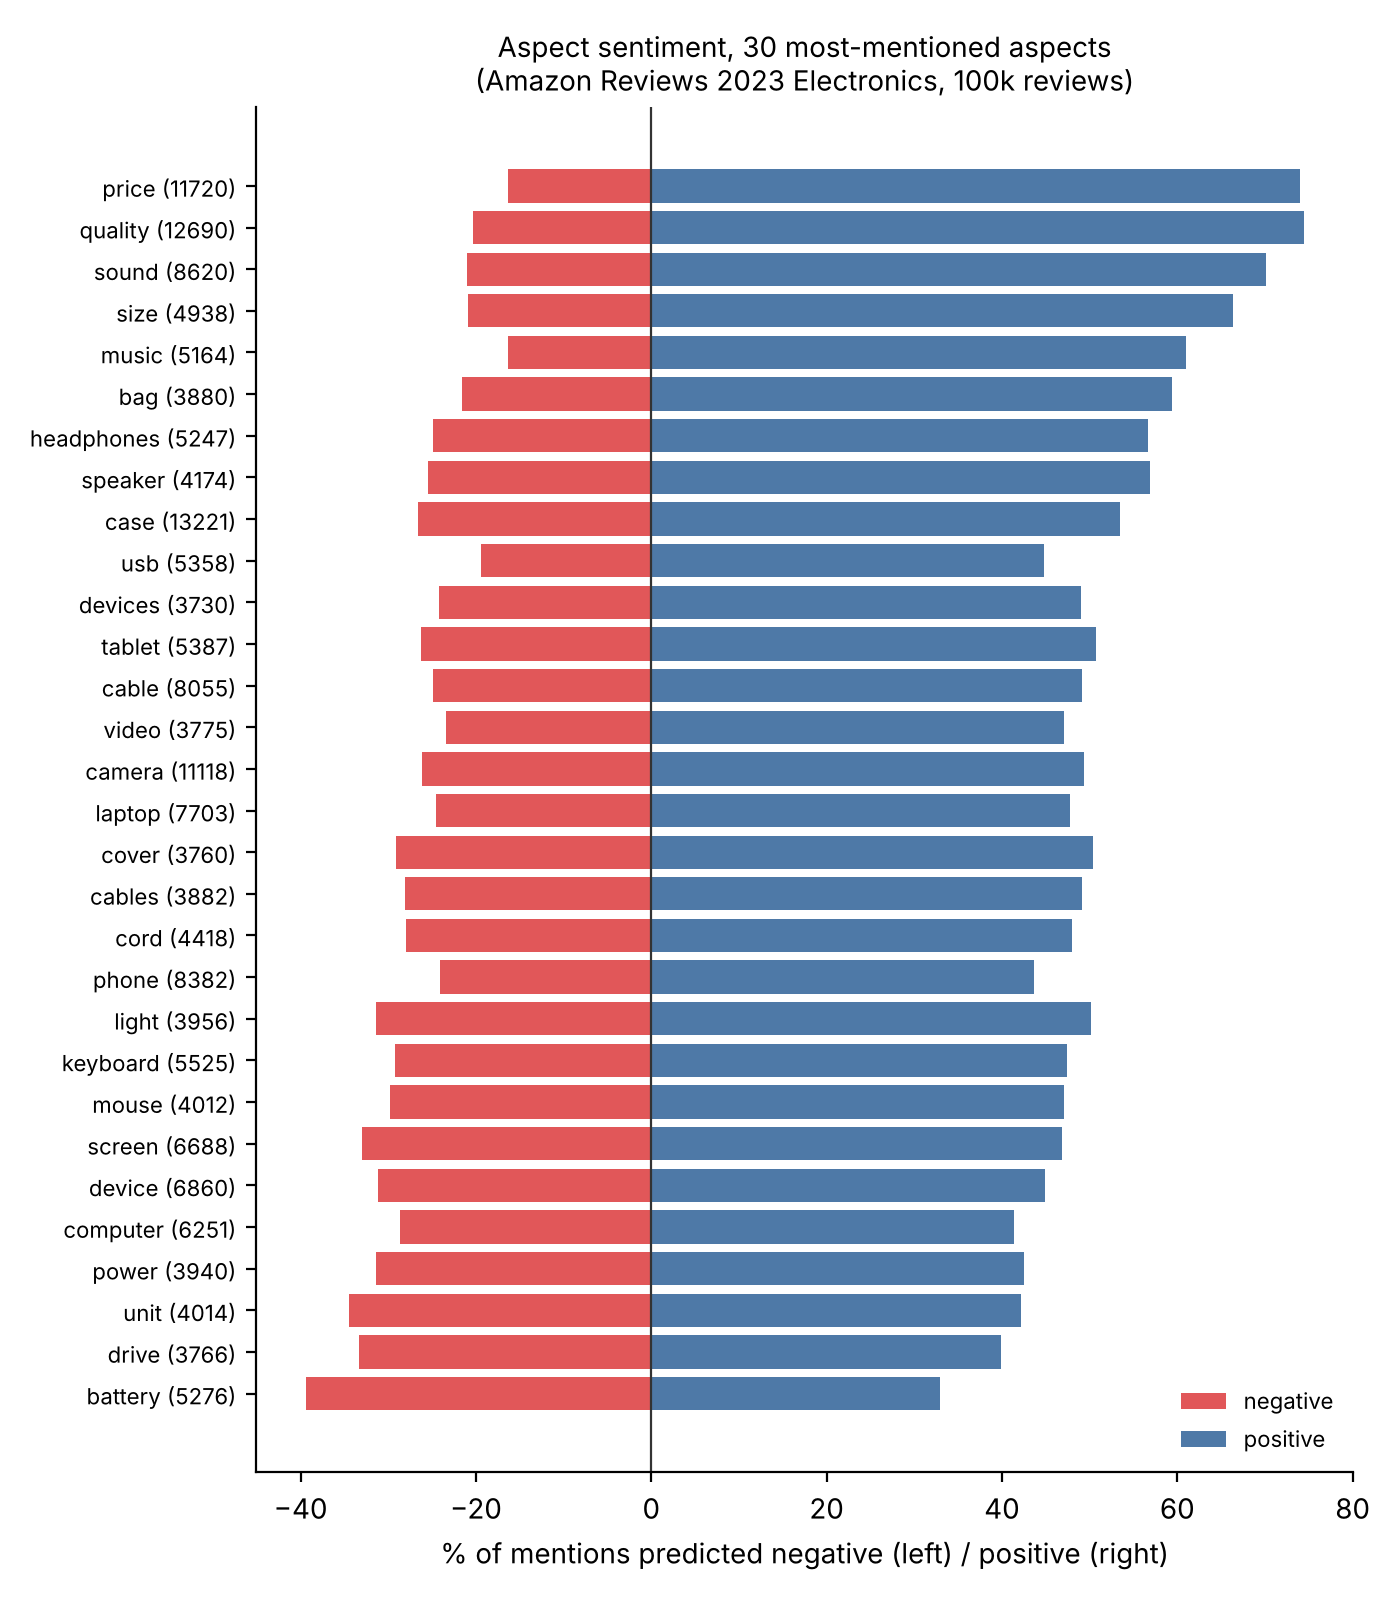
\includegraphics[width=0.78\columnwidth]{figures/top_aspects.png}
\caption{Share of mentions predicted negative and positive for the 30 most frequent aspects, GloVe R-GAT over 97k reviews. Mention counts in brackets.}
\label{fig:aspects}
\end{figure}

\begin{figure}[h]
\centering
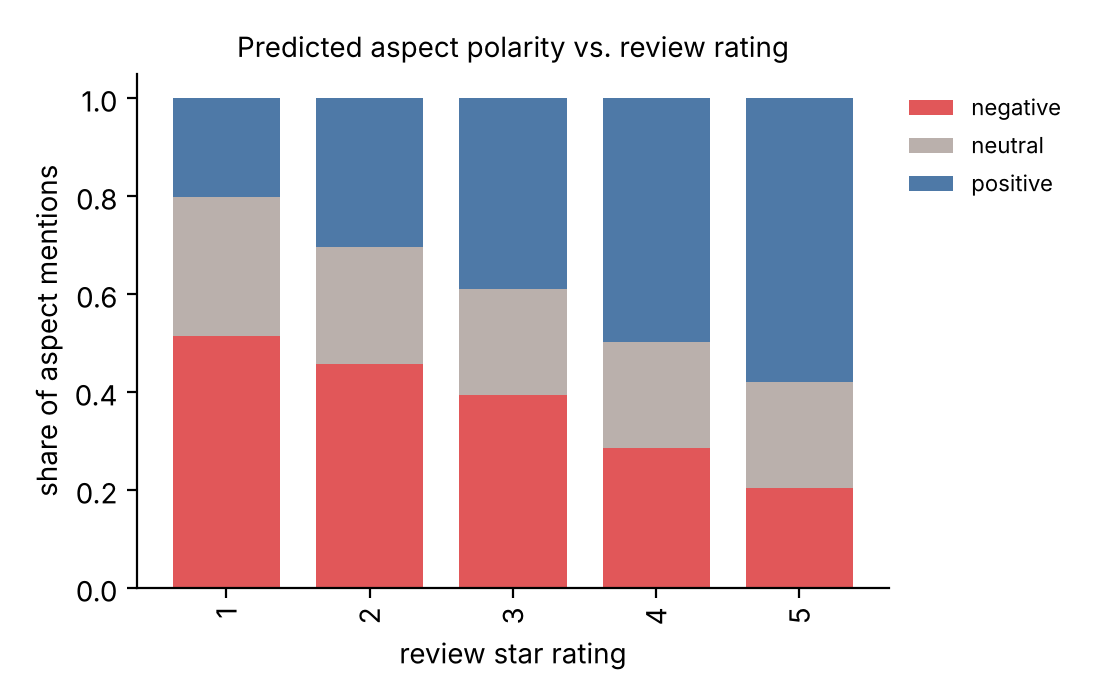
\includegraphics[width=0.72\columnwidth]{figures/polarity_by_star.png}
\caption{Predicted aspect polarity by review star rating (GloVe R-GAT, 588k mentions).}
\label{fig:stars}
\end{figure}

\section{Reproducibility}

The code is organised as a small Python package (\texttt{src/absa}) with scripts for data preparation, the experiment grid, the analysis and the corpus-scale run. Every run stores its configuration, learning curve, test metrics and per-instance predictions, and all tables in this report are produced by \texttt{scripts/analyze.py} from these files. The complete grid takes about 12 hours on four CPU cores. The processed datasets, the annotation files and an executed notebook that walks through all results are included in the repository.

\end{document}
